\documentclass[a4paper,12pt]{memoir}

\usepackage{hyperref}
\usepackage{marvosym}
\usepackage{fontawesome}

\hypersetup{
    colorlinks=true,
    linkcolor=black,
    filecolor=black,
    urlcolor=black,
}

%%%%%%%%%%%%%%%%%%%%%%%%%%%%%%%%%%%%%%%%%
% Wenneker Resume/CV
% Structure Specification File
% Version 1.1 (19/6/2016)
%
% This file has been downloaded from:
% http://www.LaTeXTemplates.com
%
% Original author:
% Frits Wenneker (http://www.howtotex.com) with extensive modifications by 
% Vel (vel@latextemplates.com)
%
% License:
% CC BY-NC-SA 3.0 (http://creativecommons.org/licenses/by-nc-sa/3.0/)
%
%%%%%%%%%%%%%%%%%%%%%%%%%%%%%%%%%%%%%%%%%

%----------------------------------------------------------------------------------------
%	PACKAGES AND OTHER DOCUMENT CONFIGURATIONS
%----------------------------------------------------------------------------------------

\usepackage{XCharter} % Use the Bitstream Charter font
\usepackage[utf8]{inputenc} % Required for inputting international characters
\usepackage[T1]{fontenc} % Output font encoding for international characters

\usepackage[top=1cm,left=1cm,right=1cm,bottom=1cm]{geometry} % Modify margins

\usepackage{graphicx} % Required for figures

\usepackage{flowfram} % Required for the multi-column layout

\usepackage{url} % URLs

\usepackage[usenames,dvipsnames]{xcolor} % Required for custom colours

\usepackage{tikz} % Required for the horizontal rule

\usepackage{enumitem} % Required for modifying lists
\setlist{noitemsep,nolistsep} % Remove spacing within and around lists

\setlength{\columnsep}{\baselineskip} % Set the spacing between columns

% Define the left frame (sidebar)
\newflowframe{0.2\textwidth}{\textheight}{0pt}{0pt}[left]
\newlength{\LeftMainSep}
\setlength{\LeftMainSep}{0.2\textwidth}
\addtolength{\LeftMainSep}{1\columnsep}
 
% Small static frame for the vertical line
\newstaticframe{1.5pt}{\textheight}{\LeftMainSep}{0pt}
 
% Content of the static frame with the vertical line
\begin{staticcontents}{1}
\hfill
\tikz{\draw[loosely dotted,color=RoyalBlue,line width=1.5pt,yshift=0](0,0) -- (0,\textheight);}
\hfill\mbox{}
\end{staticcontents}
 
% Define the right frame (main body)
\addtolength{\LeftMainSep}{1.5pt}
\addtolength{\LeftMainSep}{1\columnsep}
\newflowframe{0.7\textwidth}{\textheight}{\LeftMainSep}{0pt}[main01]

\pagestyle{empty} % Disable all page numbering

\setlength{\parindent}{0pt} % Stop paragraph indentation

%----------------------------------------------------------------------------------------
%	NEW COMMANDS
%----------------------------------------------------------------------------------------

\newcommand{\userinformation}[1]{\renewcommand{\userinformation}{#1}} % Define a new command for the CV user's information that goes into the left column

\newcommand{\cvheading}[1]{{\Huge\bfseries\color{RoyalBlue} #1} \par\vspace{.6\baselineskip}} % New command for the CV heading
\newcommand{\cvsubheading}[1]{{\Large\bfseries #1} \bigbreak} % New command for the CV subheading

\newcommand{\Sep}{\vspace{1em}} % New command for the spacing between headings
\newcommand{\SmallSep}{\vspace{0.5em}} % New command for the spacing within headings

\newcommand{\aboutme}[2]{ % New command for the about me section
\textbf{\color{RoyalBlue} #1}~~#2\par\Sep
}
	
\newcommand{\CVSection}[1]{ % New command for the headings within sections
{\Large\textbf{#1}}\par
\SmallSep % Used for spacing
}

\newcommand{\CVItem}[2]{ % New command for the item descriptions
\textbf{\color{RoyalBlue} #1}\par
#2
\SmallSep % Used for spacing
}

\newcommand{\bluebullet}{\textcolor{RoyalBlue}{$\circ$}~~} % New command for the blue bullets


%!TEX root = ./cv.tex

% Personal Info

\usepackage{tikz}

\userinformation{
	\begin{flushright}
		\begin{tikzpicture}
			\clip (0,0)  circle (2cm) ;
			\node {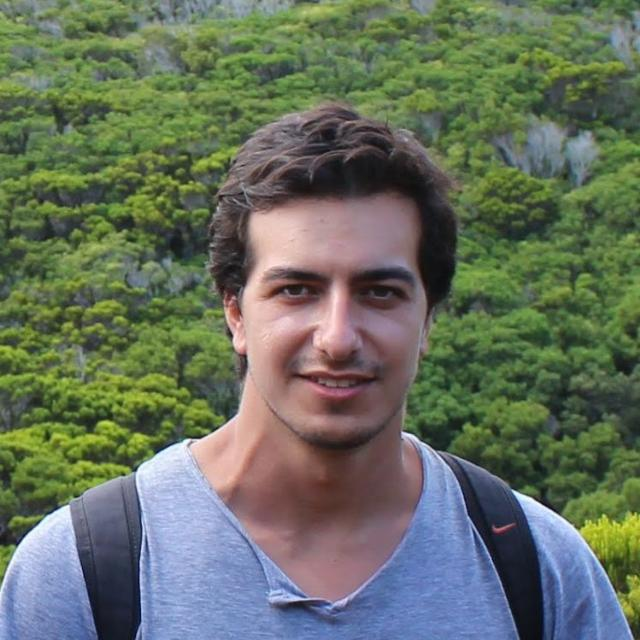
\includegraphics[width=4cm]{photo3.jpeg}}; 
		\end{tikzpicture}
		%
\includegraphics[width=0.8\columnwidth]{photo2.jpeg}\\[\baselineskip]

		\small

		André Pascoal Bento \\
		%\Letter~\href{mailto:andre.pascoal.bento@gmail.com}{andre.pascoal.bento@gmail.com} \\
		\Letter~\href{mailto:apbento@dei.uc.pt}{apbento@dei.uc.pt} \\
		\Mobilefone~(+351)~910~349~466 \\
		%\Telefon~(+351)~231~455~067 \\ 
		\faLinkedin~\href{https://www.linkedin.com/in/andre-bento/?locale=en_US}{andre-bento}
		\faGithub~\href{https://github.com/andrepbento}{andrepbento}
		\faGoogle~\href{https://scholar.google.com/citations?user=9Yl9gBwAAAAJ&hl=en}{Schollar}

		\Sep

		\textbf{Address} \\
		R. Lourenço Chaves de Almeida, Lote 2, 2.D \\
		Coimbra, 3000-249 \\
		Portugal

		\Sep

		\textbf{Communication skills} \\
		Portuguese (native) \\
		English (advanced) \\
		French (intermediate) \\
		Spanish (intermediate)

		\vfill
	\end{flushright}
}


\begin{document}

\userinformation

\framebreak

\cvheading{André Bento}

\cvsubheading{PhD Student @ CISUC | Assistant Professor @ University of Coimbra}

\aboutme{About}{
    André Bento is a researcher at the Centre for Informatics and Systems at the University of Coimbra.
    He is also a PhD student in Informatics Engineering and an invited professor at the University of Coimbra.
    He received his B.Sc. degree from the Coimbra Institute of Engineering and his M.Sc. degree from the University of Coimbra, both in Informatics Engineering.
    Besides studying and working, André Bento is a regular swimmer and enjoys cycling, running and long walks in nature.
    As an enthusiast of distributed systems and cloud-based solutions, he is constantly looking for opportunities to improve and learn new methods and technologies.
}

\CVSection{Education}

\CVItem{2019 - Present, University of Coimbra}{Ph.D. in Informatics Engineering
\\\emph{Thesis: Optimizing Availability and Resource Utilization of Cloud Services}
}

\CVItem{2017 - 2019, University of Coimbra}{M.Sc. in Informatics Engineering
\\\emph{Thesis: Observing and Controlling Performance in Microservices}}

\CVItem{2014 - 2017, Coimbra Institute of Engineering (ISEC)}{B.Sc. in Informatics Engineering}

\Sep

\CVSection{Experience}

\CVItem{Sep 2021 - Present, \textit{Invited Professor}, University of Coimbra}{
    Teaching practical laboratory classes on Distributed Systems and Systems Integration.
}

\CVItem{Sep 2019 - Present, \textit{Researcher}, CISUC - Centre for Informatics and Systems (University of Coimbra)}{
    Research methods and techniques to improve the availability and reliability of microservices using anomaly detection and root-cause analysis.\\
    Working with technologies such as Docker, Kubernetes, Terraform, Ansible, AWS, Istio, Grafana, Prometheus, Jaeger, Kiali, and others.
}

\CVItem{Sep 2018 - Jul 2019, \textit{Research Intern}, CISUC - Centre for Informatics and Systems (University of Coimbra)}{
    Researched Microservices, Observability and Performance Monitoring using Metrics, Logs and Distributed Tracing.
}

\CVItem{Feb 2017 - Jul 2017, \textit{Software Engineer Intern}, WIT Software, S.A.}{
    Developed a Mobile AR Prototype with digital filters and image manipulation features, focusing on enhanced user content creation, e.g., Selfies, Stickers, Photo Effects/Filters, Emojis and Drawings, in an exploratory Android and iOS project.
}

\CVItem{Oct 2016 - Jun 2017, \textit{Scratch Teacher Assistant}, CASPAE 10}{
    Taught problem-solving techniques using the Scratch programming language to children attending the 3rd and 4th grades of primary school.
}

\Sep

\clearpage

\userinformation

\framebreak


\CVItem{Nov 2015 - Mar 2016, \textit{Math Applied to Engineer Teacher -- Volunteer}, CeAMatE}{
    Taught mathematics to pre-degree, CTeSP and Engineering students.
}

\CVItem{May 2014 - Jul 2014, \textit{Accountant Technician Intern}, Caixa de Crédito Agrícola Mútuo de Mira - C.R.L.}{
    Bank accountant, bank organization and bank day-to-day work.
}

\CVItem{May 2013 - Jun 2013, \textit{Accountant Technician Intern}, Caixa de Crédito Agrícola Mútuo de Cantanhede - C.R.L.}{
    Bank accountant, bank organization and bank day-to-day work.
}

\Sep

\CVSection{Publications}

\begin{enumerate}
	\item Andre Bento, Filipe Araujo, Luís Paquete, and Raul Barbosa. 
	Optimal Scaling of Cloud Services. Submitted to an International Journal.
	% \item \td{Andre Bento, Filipe Ribeiro, António Ferreira, Filipe Araujo, and 
	% Raul Barbosa. Modeling the Availability of Cloud Service Replicas. [WIP 
	% submitted to European Dependable Computing Conference [EDCC 2025]]}.
	\item Andre Bento, Filipe Araujo, and Raul Barbosa. Cost-availability aware
	scaling: Towards optimal scaling of cloud services. Journal of Grid 
	Computing, 21(4):80, 2023.% [Rank Q1 by Scimago Journal \& Country Rank].
	\item Gonçalo Baptista, Jaime Correia, Andre Bento, Joao Soares, Antonio 
	Ferreira, Joao Duraes, Raul Barbosa, and Filipe Araujo. Defektor: An 
	extensible tool for fault injection campaign management in microservice 
	systems. In Proceedings of the 38th ACM/SIGAPP Symposium on Applied 
	Computing, SAC'23, page 184-187, New York, NY, USA, 2023.% Association for
	%Computing Machinery. (Poster paper presented in conference at Tallinn,
	%Estonia, March 27-31, 2023).% [Rank B by ERA]. 
	\item Stanley Lima, Filipe Araujo, Miguel de Oliveira Guerreiro, Jaime 
	Correia, Andre Bento, and Raul Barbosa. Efficient causal access in 
	geo-replicated storage systems. Journal of Grid Computing, 21(1):8, 2023.
	%[Rank Q1 by Scimago Journal \& Country Rank].
	% \item Stanley Lima, Filipe Araujo, Miguel de Oliveira Guerreiro, Jaime 
	% Correia, Andre Bento, and Raul Barbosa. Optimal causal access in 
	% geo-replicated storage systems. 2022. Research Square - \td{Preprint}.
	\item Andre Bento, Joao Soares, António Ferreira, Joao Duraes, José 
	Ferreira, Rita Carreira, Filipe Araujo, and Raul Barbosa. Bi-objective 
	optimization of availability and cost for cloud services. In 2022 IEEE 21st 
	International Symposium on Network Computing and Applications (NCA), volume 
	21, pages 45-53. IEEE, 2022.% [Rank A by ERA].
	\item Andre Bento, Jaime Correia, Joao Duraes, João Soares, Luís Ribeiro,
	António Ferreira, Rita Carreira, Filipe Araujo, and Raul Barbosa. A layered 
	framework for root cause diagnosis of microservices. In 2021 IEEE 20th 
	International Symposium on Network Computing and Applications (NCA), 
	pages 1-8. IEEE, 2021.% [Rank A by ERA].
	\item João Tomás, André Bento, João Soares, Luís Ribeiro, António Ferreira,
	Rita Carreira, Filipe Araújo, and Raul Barbosa. Autonomic service operation 
	for cloud applications: Safe actuation and risk management. In Dependable 
	Computing-EDCC 2021 Workshops: DREAMS, DSOGRI, SERENE 2021, Munich, Germany, 
	September 13, 2021, Proceedings 17, pages 39-46. Springer, 2021.% [Rank B2 by
	% Qualis].
	\item Sara Silva, Jaime Correia, Andre Bento, Filipe Araujo, and Raul 
	Barbosa. $\mu$Viz: Visualization of microservices. In 2021 25th 
	International Conference Information Visualisation (IV), pages 120-128. 
	IEEE, 2021.% [Rank B by ERA].
	\item Andre Bento, Jaime Correia, Ricardo Filipe, Filipe Araujo, and Jorge 
	Cardoso. Automated analysis of distributed tracing: Challenges and research
	directions. Journal of Grid Computing, 19:1-15, 2021.% [Rank Q1 by Scimago 
	%Journal \& Country Rank].
\end{enumerate}

\Sep

\clearpage

\userinformation

\framebreak

\CVSection{Grants and Projects}

\begin{itemize}
    \item \textbf{PhD grant} - Foundation for Science and Technology (FCT) Grant number BD.06012.2021. (Dec 2021 - Jul 2025)
    \item \textbf{ROAR-NET} - Randomised Optimisation Algorithms Research Network (CA22137). Funded by COST. (2023 - 2025)
    \item \textbf{AESOP} - Autonomic Service Operation. Funded by P2020-31/SI/2017, No. 040004. (2019 - 2022) 
\end{itemize}

\Sep

\CVSection{Interests}

\CVItem{Professional}{Cloud computing, Microservices, Monitoring, Observability, Tracing, Anomaly Detection, Self-adaptive Systems, Optimal Scaling, Data analysis, Machine learning, Programming languages and Software Engineering.}

\CVItem{Personal}{Travelling, Cycling, Running, Long walks, Swimming, Trekking, Learning to play Guitar and having fun with family and friends.}

\end{document}
